\def\mytitle{OPTIMIZATION}
\def\myauthor{VAMSI SUNKARI}
\def\contact{vamsisunkari9849@gmail.com}
\def\mymodule{Future Wireless Communication (FWC)}
\documentclass[10pt, a4paper]{article}
\usepackage[a4paper,outer=1.5cm,inner=1.5cm,top=1.75cm,bottom=1.5cm]{geometry}
\twocolumn
\usepackage{setspace}
\usepackage{graphicx}
\graphicspath{{./images/}}
\usepackage[colorlinks,linkcolor={black},citecolor={blue!80!black},urlcolor={blue!80!black}]{hyperref}
\usepackage[parfill]{parskip}
\usepackage{lmodern}
\usepackage{tikz}
 \usepackage{physics}
%\documentclass[tikz, border=2mm]{standalone}
\usepackage{karnaugh-map}
\usepackage{tabularx}
\usetikzlibrary{calc}
\usepackage{amsmath}
\usepackage{amssymb}
\renewcommand*\familydefault{\sfdefault}
\usepackage{watermark}
\usepackage{lipsum}
\usepackage{xcolor}
\usepackage{listings}
\usepackage{float}
\usepackage{titlesec}
\providecommand{\mtx}[1]{\mathbf{#1}}
\titlespacing{\subsection}{1pt}{\parskip}{3pt}
\titlespacing{\subsubsection}{0pt}{\parskip}{-\parskip}
\titlespacing{\paragraph}{0pt}{\parskip}{\parskip}
\newcommand{\figuremacro}[5]{//
    \begin{figure}[#1]
        \centering
        \includegraphics[width=#5\columnwidth]{#2}
        \caption[#3]{\textbf{#3}#4}
        \label{fig:#2}
    \end{figure}
}
\newcommand{\myvec}[1]{\ensuremath{\begin{pmatrix}#1\end{pmatrix}}}
\let\vec\mathbf
\lstset{
frame=single, 
breaklines=true,
columns=fullflexible
}

\title{\mytitle}
\author{\myauthor\hspace{1em}\\\contact\\FWC22040\hspace{6.5em}IITH\hspace{0.5em}\mymodule\hspace{6em}ASSIGN-8}
\date{}
\begin{document}
 \maketitle
 \tableofcontents

\section{Construction}
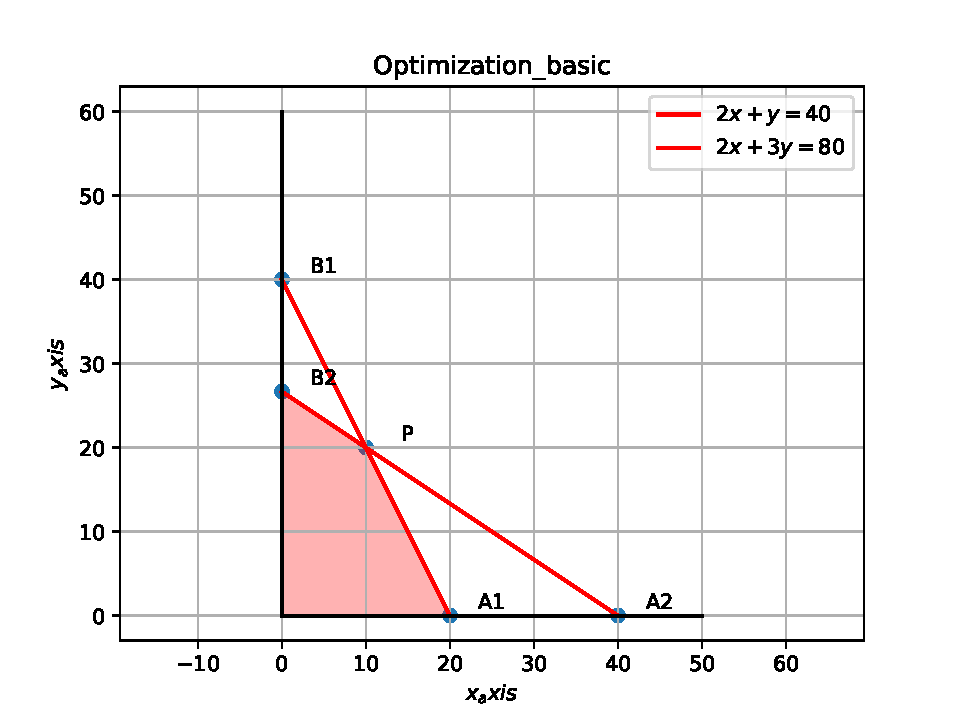
\includegraphics[scale=0.5]{im.pdf}

\section{Problem}
A manufacturer has employed 5 skilled men and 10 semi-skilled men and makes two models A and B of an article. The making of one item of model A requires 2 hours work by a skilled man and 2 hours work by a semi-skilled man. One item of model B requires 1 hour by a skilled man and 3 hours by a semi-skilled man. No man is expected to work more than 8 hours per day. The manufacturers profit on an item of model A is Rs. 15 and on an item of model B is Rs. 10. How many of items of each model should be made per day in order to maximize daily profit? Formulate the above LPP and solve it graphically and find the maximum profit.
\section{Solution}
Consider,
\begin{tabular}{|c|c|}
 \hline
 \textbf{Parameter}&\textbf{Value}\\
 \hline
 $\vec{c}$ & $\myvec{15\\10}$ \\
 \hline
 $\vec{x}$ & $\myvec{x\\y}$ \\
 \hline
 $\vec{p}$ & $\myvec{2&1 \\ 2&3 \\ 0&-1 \\ -1&0}$ \\
 \hline
\end{tabular}\\

Objective function:
\begin{equation}
 \vec{z} = \max_{x}\vec{c}^T\vec{x}
\end{equation}
Constraints:
\begin{equation}
2x + y\le 40
\end{equation}
\begin{equation}
2x + 3y \le 80
\end{equation}
\begin{equation}
-x \le 0
\end{equation}
\begin{equation}
-y \le 0
\end{equation}
writing all the constraints in matrix form:
\begin{equation}
\vec{p^T}\vec{x} \preceq \vec{q}
\end{equation}
\begin{equation}
\myvec{2&1 \\2&3 \\ 0&-1 \\ -1&0}x \preceq \myvec{40 \\ 80 \\ 0 \\ 0 }
\end{equation}
By providing the objective function and constraints to cvxpy, we get the optimal solution for z
\\
\textbf{cvxpy code}

from cvxpy code,\\
The optimal solution is $\vec{z} = \myvec{10 \\ 20}$

\end{document}
